\documentclass[11pt,a4paper]{article}

% ---------- Packages ----------
\usepackage{xcolor}
\usepackage{graphicx}
\usepackage{longtable}
\usepackage{array}
\usepackage{tabularx}
\usepackage{textcomp}
\usepackage[colorlinks=true,linkcolor=vigilaccent,urlcolor=vigilaccent,pdfencoding=auto]{hyperref}
\usepackage{tikz}
\usetikzlibrary{arrows.meta,positioning,shapes.geometric,fit,calc}
% Manual page margins (geometry replacement)
\setlength{\topmargin}{-1.5cm}
\setlength{\headheight}{0.5cm}
\setlength{\headsep}{0.3cm}
\setlength{\textwidth}{16.5cm}
\setlength{\textheight}{24.5cm}
\setlength{\oddsidemargin}{0cm}
\setlength{\evensidemargin}{0cm}
% Captions use default styling
% Section title style (titlesec replacement — manual formatting in \sectionrule)
% List spacing (enumitem replacement — manual \vspace used instead)
% Book-quality tables (booktabs replacement — \hline used instead)

% ---------- Colors ----------
\definecolor{vigilblue}{HTML}{0A1628}
\definecolor{vigilaccent}{HTML}{0E7490}
\definecolor{vigilamber}{HTML}{F59E0B}
\definecolor{vigilred}{HTML}{EF4444}
\definecolor{vigilgreen}{HTML}{22C55E}
\definecolor{vigilcyan}{HTML}{06B6D4}
\definecolor{vigilgray}{HTML}{6B7280}
\definecolor{vigilpurple}{HTML}{8B5CF6}
\definecolor{softblue}{HTML}{0E7490}
\definecolor{lightbg}{HTML}{F1F5F9}
\definecolor{rowtint}{HTML}{EEF4FA}
\definecolor{deepnavy}{HTML}{07111F}
\definecolor{panelblue}{HTML}{E6F6FA}
\definecolor{softamber}{HTML}{FFF7E6}

% Section styling is done via \sectionrule command

% ---------- Table helpers ----------
\renewcommand{\arraystretch}{1.25}
\newcolumntype{Y}{>{\raggedright\arraybackslash}X}

% Screenshot convenience command
\newcommand{\shot}[2]{%
  \begin{figure}[!ht]\centering
    \includegraphics[width=\linewidth,height=0.62\textheight,keepaspectratio]{screenshots/#1}%
    \caption{#2}
  \end{figure}}

\newcommand{\sectionrule}{\noindent{\color{vigilaccent}\rule{0.22\linewidth}{2.2pt}}{\color{vigilaccent!30}\rule{0.78\linewidth}{0.6pt}}\par\vspace{4pt}}
\newcommand{\statcard}[3]{%
  \fcolorbox{vigilaccent!35}{lightbg}{\begin{minipage}[c][1.9cm][c]{2.75cm}\centering
    {\Large\bfseries\color{vigilblue} #1}\\[-1pt]
    {\scriptsize\bfseries\color{vigilaccent} #2}\\[-1pt]
    {\tiny\color{vigilgray} #3}
  \end{minipage}}}
\newcommand{\featurepill}[1]{\fcolorbox{vigilaccent!30}{panelblue}{\strut\hspace{4pt}\scriptsize\bfseries\color{vigilblue}#1\hspace{4pt}}}
\newcommand{\judgecallout}[2]{%
  \begin{center}
  \fcolorbox{vigilaccent}{lightbg}{\begin{minipage}{0.92\linewidth}
  {\bfseries\color{vigilblue}#1}\par\vspace{3pt}{#2}
  \end{minipage}}
  \end{center}}

\begin{document}

% ============================================================
% PAGE 1 — TITLE PAGE
% ============================================================
\begin{titlepage}
\thispagestyle{empty}
\begin{tikzpicture}[remember picture,overlay]
  \fill[deepnavy] (current page.south west) rectangle (current page.north east);
  \fill[vigilaccent!22] ([xshift=-2cm,yshift=2cm]current page.north east) circle (5.4cm);
  \fill[vigilcyan!16] ([xshift=1.4cm,yshift=-1.4cm]current page.south west) circle (5.1cm);
  \draw[vigilaccent!35,line width=0.8pt] ([xshift=1.1cm,yshift=-1.1cm]current page.north west) rectangle ([xshift=-1.1cm,yshift=1.1cm]current page.south east);
  \draw[vigilcyan!20,line width=0.4pt] ([xshift=1.45cm,yshift=-1.45cm]current page.north west) rectangle ([xshift=-1.45cm,yshift=1.45cm]current page.south east);
\end{tikzpicture}
\centering
\vspace*{0.6cm}

{\color{vigilcyan}\rule{\linewidth}{1.5pt}}
\vspace{0.6cm}

{\Huge\bfseries\color{white} VigilAI}\\[10pt]
{\large\bfseries\color{vigilcyan} Software-Only AI Enforcement for Bengaluru Traffic Images}\\[6pt]
{\normalsize\itshape\color{white!85} AI detects. Officers decide. Evidence stays auditable.}

\vspace{0.8cm}
{\color{vigilcyan!60}\rule{0.5\linewidth}{0.6pt}}
\vspace{0.5cm}

{\large\bfseries\color{white} Flipkart GridLock 2.0 \,\textbullet\, Round 2 \,\textbullet\, Track 3}\\[4pt]
{\normalsize\color{white!80} June 21, 2026}

\vspace{0.9cm}

% Headline stats
\statcard{7/7}{Violations}{problem-statement coverage}\hspace{0.25cm}
\statcard{$<$3\,s}{Latency Target}{upload to response}\hspace{0.25cm}
\statcard{2.8\,GB}{Peak VRAM Plan}{4\,GB-GPU strategy}\hspace{0.25cm}
\statcard{12}{Console Pages}{operator workflow}

\vspace{0.5cm}
{\small\itshape\color{white!88}
Processes existing CCTV images, citizen reports, and video clips; detects violations, reads license plates, and generates officer-reviewable evidence.
}

\vspace{0.55cm}
\featurepill{Detection}\hspace{3pt}\featurepill{OCR}\hspace{3pt}\featurepill{Evidence Hashing}\hspace{3pt}\featurepill{Officer Review}\hspace{3pt}\featurepill{Analytics}\hspace{3pt}\featurepill{Map}\hspace{3pt}\featurepill{Video}\hspace{3pt}\featurepill{Citizen Reports}

\vfill

% Team
{\color{vigilcyan!60}\rule{0.5\linewidth}{0.6pt}}
\vspace{0.4cm}

{\normalsize\bfseries\color{white} Team}\\[6pt]
\fcolorbox{vigilcyan}{white}{\begin{minipage}{0.88\linewidth}\centering
{\large\bfseries\color{vigilblue} Vedant Tong \;\textbullet\; Vinit Gaikwad \;\textbullet\; Jayashri Utrankar \;\textbullet\; Tanishq Agarwal}
\end{minipage}}

\vspace{0.2cm}
{\small\color{white!80}\url{https://github.com/VTongTV/flipkart-gridlock-2.0-round-II.git}}

\vspace{0.6cm}
{\color{vigilcyan}\rule{\linewidth}{1.5pt}}
\end{titlepage}

% ============================================================
% PAGE 2 — EXECUTIVE SUMMARY FOR JUDGES
% ============================================================
\thispagestyle{empty}
{\Large\bfseries\color{vigilblue} Summary}
\vspace{4pt}\\
{\color{vigilaccent}\rule{\linewidth}{1pt}}
\vspace{6pt}

\noindent\textbf{VigilAI is a working traffic-violation analysis prototype that turns traffic images into detected violations, license-plate OCR, officer review records, evidence images, analytics, and challan-ready PDFs.}

\vspace{6pt}

\noindent The system is built around the exact problem statement: preprocess difficult road images, detect vehicles and road users, classify traffic violations, extract plates, create annotated evidence, support reporting, and evaluate model and system performance.

\vspace{8pt}

\begin{center}
\begin{tabular}{@{}p{3.5cm}p{9cm}@{}}
\hline
\textbf{What judges asked for} & \textbf{What VigilAI demonstrates} \\
\hline
Image preprocessing & CLAHE, denoising, and gamma correction for CCTV-style inputs \\
Vehicle / road-user detection & YOLOv8n-based person, vehicle, motorcycle, bus, truck, bicycle, helmet, and no-helmet detection \\
Violation detection & All seven listed violation categories are represented: helmet, seatbelt, triple riding, wrong-side, stop-line, red-light, and illegal parking \\
Violation classification & Violation type, confidence score, severity, MV Act reference, and review status \\
License plate recognition & Plate detection, RapidOCR on CPU, Indian plate-format validation, and manual-review fallback \\
Evidence generation & Annotated evidence image, timestamp, metadata, SHA-256 hash, audit trail, and challan PDF generation \\
Analytics and reporting & Dashboard, searchable violations, trend charts, heatmap, map view, camera view, and ROI calculator \\
Efficiency and scalability & VRAM-aware model loading planned for a 4\,GB RTX 3050; target end-to-end response under 3 seconds \\
\hline
\end{tabular}
\end{center}

\vspace{8pt}

\noindent\textbf{What makes the prototype judge-friendly:} it is not only an object detector. It includes the full enforcement workflow: image or video intake $\rightarrow$ AI detection $\rightarrow$ OCR $\rightarrow$ evidence generation $\rightarrow$ officer approval / rejection $\rightarrow$ analytics and reporting.

\vspace{8pt}

\judgecallout{Winning thesis}{VigilAI turns traffic images into officer-verified, tamper-evident enforcement records using practical computer vision and a police-oriented command center.}

\vfill
\begin{center}
\color{vigilblue}\bfseries AI detects. Officers decide. Evidence stays auditable.
\end{center}
\newpage

% ============================================================
% PAGE 3 — TABLE OF CONTENTS
% ============================================================
\thispagestyle{empty}
{\Large\bfseries\color{vigilblue} Contents}
\vspace{4pt}\\
{\color{vigilaccent}\rule{\linewidth}{1pt}}
\vspace{6pt}
\renewcommand{\contentsname}{\vspace{-2.2em}}
\tableofcontents
\thispagestyle{empty}
\vfill
\begin{center}
\small\itshape VigilAI — built for the Bengaluru Traffic Police, designed for every Indian city.
\end{center}
\newpage

\setcounter{page}{1}

% ============================================================
% SECTION 1 — THE PROBLEM
% ============================================================
\section{The Problem}
\sectionrule

Bengaluru is one of the most congested cities on earth, yet its traffic enforcement runs on two very different gears. A small fraction of junctions are modern and automated; the overwhelming majority are not. This asymmetry is the single biggest reason that routine violations — no helmet, triple riding, wrong-side driving, illegal parking — continue unchecked, every single day, on hundreds of roads across the city.

\subsection{A City Split in Two}

The Bengaluru Traffic Police (BTP) operates roughly \textbf{575 traffic junctions}. Of these, only about \textbf{75 junctions} carry AI-assisted, contactless enforcement systems. The remaining \textbf{500+ junctions} — covering the vast majority of the city's road network — still depend on an officer standing at the corner, watching traffic and waving down offenders by hand.

This is not a marginal gap. It is the difference between a junction that issues hundreds of evidence-backed challans a week and a junction that issues almost none.

\begin{itemize}
  \item \textbf{Coverage gap.} Only $\sim$13\% of junctions have AI enforcement. At the other 87\%, violations during off-peak hours, at night, or in bad weather are effectively invisible.
  \item \textbf{Capital barrier.} Upgrading a single junction to a proprietary AI-enforcement system costs \textbf{Rs.\,2--5 lakh} in dedicated hardware, servers, and integration. Scaling that across 500+ junctions is a multi-year, multi-crore capital project that has simply not happened.
  \item \textbf{Manual bottleneck.} A human officer can observe, note, and issue a challan for perhaps a few dozen violations per shift. An AI pipeline can screen thousands of frames. Manual review is empirically \textbf{$\sim$3.2$\times$ slower} than AI-assisted review — and far more fatiguing.
  \item \textbf{Evidence that is hard to act on.} A raw photo is not the same as an enforceable record. Police need timestamps, officer review, plate information, violation category, metadata, and integrity checks before a violation can be trusted downstream.
\end{itemize}

\subsection{Why the Gap Persists}

The reason 500+ junctions remain manual is not a lack of will — it is a lack of a \emph{deployable, affordable} system. Today's options force an all-or-nothing choice: either buy a complete, expensive, vendor-locked hardware stack per junction, or rely on a human. There is no middle path that turns the city's \emph{existing} CCTV cameras — already installed at most major junctions — into enforcement-grade sensors at near-zero marginal cost.

Meanwhile, three enormous, underused streams of evidence sit completely untapped:

\begin{itemize}
  \item \textbf{Citizen smartphones.} Every commuter with a phone is a potential mobile enforcement camera, yet there is no trusted channel to submit violations that police can actually act on.
  \item \textbf{Social media.} Thousands of traffic violations are photographed and posted publicly every day. No enforcement system in India currently processes this evidence at scale.
  \item \textbf{Evidence packaging.} Even when raw evidence exists, the gap between ``a photo of a violation'' and ``an annotated, MV-Act-referenced, tamper-evident evidence record'' is large.
\end{itemize}

\subsection{The Cost of Doing Nothing}

The status quo is not neutral. Every un-enforced junction normalises violation, erodes road safety, and forfeits legitimate fine revenue that funds further enforcement. Two-wheeler riders without helmets, triple-loaded motorcycles, and wrong-side vehicles are not just administrative nuisances — they are the leading contributors to urban road fatalities. An enforcement system that cannot see 87\% of the city cannot meaningfully change driver behaviour.

\vspace{4pt}
\begin{quote}
\color{vigilaccent}\itshape The core problem is therefore not detection technology itself — it is \textbf{coverage, cost, and trust}. VigilAI is built to solve exactly these three.
\end{quote}

\shot{02-problem.png}{The Problem, as presented in the VigilAI command console.}

% ============================================================
% SECTION 2 — THE SOLUTION
% ============================================================
\section{The Solution}
\sectionrule

VigilAI is a software-first enforcement layer designed to work with existing traffic images and CCTV-style feeds. It takes the frames a city already captures and turns them into detected violations, read license plates, and officer-reviewable evidence packages, all shown through a purpose-built command center designed for police officers, not engineers.

The single design principle: \textbf{make the enforcement workflow practical on existing imagery and low-cost compute before assuming expensive junction hardware upgrades.}

\subsection{Three-Phase Enforcement Loop}

\begin{itemize}
  \item \textbf{Phase 1 — AI Detects.} YOLOv8 models process uploaded traffic images and video-extracted frames, detecting \textbf{7 violation types}: helmet non-compliance, triple riding, wrong-side driving, illegal parking, seatbelt non-compliance, stop-line violation, and red-light violation. License plates are read via OCR.
  \item \textbf{Phase 2 — Officers Verify.} Flagged violations land in a command-center dashboard. Officers review the annotated evidence and \emph{approve or reject each one}. The AI assists; it never replaces human judgement. This is deliberate — it protects against wrongful challans and keeps a human accountable for every ticket.
  \item \textbf{Phase 3 — Evidence Package.} Approved violations are packaged into annotated evidence images with \textbf{SHA-256 hashes}, metadata, MV Act section references, fine amounts, and challan PDF output — ready for officer-side review and downstream enforcement workflows.
\end{itemize}

\shot{03-solution.png}{The three-phase enforcement loop: AI Detects $\rightarrow$ Officers Verify $\rightarrow$ Court-Ready Evidence.}

\subsection{The Three-Pillar Evidence Architecture}

The headline insight of VigilAI is that no enforcement system in India unifies three complementary evidence streams into a single workflow. VigilAI does — and each pillar is a shipped endpoint in the running system, not a roadmap item.

\begin{itemize}
  \item \textbf{Pillar I — CCTV / Image Analysis} (\texttt{POST /api/v1/detect}). Process traffic images through the full pipeline: preprocessing, object detection, violation logic, plate OCR, evidence annotation, persistence, and timing breakdown. The same system also accepts \emph{video clips} frame-by-frame (\texttt{POST /api/v1/video/detect}).
  \item \textbf{Pillar II — Citizen Reporting} (\texttt{POST /api/v1/citizen/detect}). Citizens can submit violation photos through a privacy-first interface. The response is deliberately redacted — no plate text, fine amount, MV Act section, or evidence hash is shown to the submitter.
  \item \textbf{Pillar III — Social-Media Intelligence Prototype} (\texttt{GET /api/v1/scraper/feed}). The console demonstrates how public traffic posts could be triaged with source attribution and routed into the same review mindset. In the current prototype, this is a mock feed rather than a live scraper.
\end{itemize}

The image, video, and citizen channels use the same detection and evidence principles. The social-media page demonstrates the intended intelligence workflow with mock data, keeping the prototype honest while still showing the product direction.

\subsection{Why It Works on a\texorpdfstring{\,}{ }4\texorpdfstring{\,}{ }GB GPU}

A major practical barrier to city-scale AI enforcement is hardware cost. VigilAI is engineered to run three YOLOv8n models plus RapidOCR entirely on a single consumer-grade RTX 3050 (4\,GB VRAM) through VRAM-aware on-demand model loading: the COCO and helmet models stay resident, the plate model loads only when a vehicle is detected and unloads immediately after inference, and OCR runs on CPU. Peak VRAM stays under \textbf{2.8\,GB}. This is what makes per-junction edge deployment economically viable.

\subsection{Beyond the Pillars — The Extended Command Surface}

Around the three-pillar detection engine, VigilAI ships an integrated set of operational modules that turn raw detections into a complete control-room product. Each is a live page in the running console.

\begin{itemize}
  \item \textbf{Live Tracking} (\texttt{GET /api/v1/tracking/overview}). A command-center overview of monitored junction status, last-hour violations, last violation type, and aggregate alerts. In the prototype this view is backed by demo tracking data.
  \item \textbf{AI Image Forensics} (\texttt{POST /api/v1/deepfake/analyze}). A separate integrity-check endpoint scores five heuristic signal classes — texture variance, saturation anomaly, edge coherence, centre-region symmetry, and noise uniformity — to flag suspicious submitted images for manual caution.
  \item \textbf{Synthetic Edge-Case Generator} (\texttt{/dashboard/generator}). A frontend demo for exploring rare traffic scenarios such as rain, night, fog, crowded pillion riding, and unusual camera angles. It helps communicate the planned robustness workflow without claiming a completed training loop.
\end{itemize}

\subsection{What Makes It Court-Admissible}

Every violation produces a tamper-evident evidence package designed around electronic-record integrity needs: an annotated image hashed with \textbf{SHA-256} immediately on generation, metadata (timestamps, confidence scores, violation type, review actions), automatic MV Act section + fine assignment, and a challan PDF on approval. Any later image change alters the hash, making tampering detectable.

\shot{04-ai-engine.png}{The multi-model detection engine, shown in the console's AI Engine view.}

\shot{09-architecture.png}{The five-layer system architecture: Frontend, API, AI Engine, Database, and Insights.}

\subsection{Novel Contributions}

VigilAI introduces several original ideas beyond standard object detection:

\begin{itemize}
  \item \textbf{Head-region spatial association} for helmet detection — uses the top 30\% of each person bounding box as a head-region proxy and matches it to helmet / no-helmet detections via IoU. This eliminates the need for a separate head detector and saves $\sim$0.8\,GB VRAM.
  \item \textbf{Three-channel enforcement workflow} combining image/video detection, privacy-redacted citizen reporting, and a social-media intelligence prototype in one console.
  \item \textbf{VRAM-aware on-demand loading} — three models in 4\,GB.
  \item \textbf{Image-forensics utility} — a separate endpoint and UI score suspicious submissions using texture, saturation, edge, symmetry, and noise heuristics.
  \item \textbf{Synthetic edge-case planning UI} — a shipped frontend page that shows how rare scenarios can be catalogued for future testing and augmentation.
  \item \textbf{Confidence-tier system} — every violation is honestly bucketed into Primary, Heuristic, or Best-effort tiers with documented confidence discounts, so the decision pipeline is auditable rather than opaque.
\end{itemize}

\shot{05-how-it-works.png}{How it works: the Challenge $\rightarrow$ Intelligence $\rightarrow$ Impact flow.}

\shot{06-features.png}{Key differentiators, organised into operational clusters.}

\shot{07-impact.png}{City-wide impact: retrofit coverage and projected revenue recovery.}

% ============================================================
% SECTION 3 — PROPOSED APPROACH (DETAILED)
% ============================================================
\section{Proposed Approach}
\sectionrule

\subsection{Adaptive Preprocessing}

Every input frame passes through three sequential OpenCV operations before inference, so that a cheap, aging CCTV sensor produces a clean, normalised image the models can actually read.

\begin{itemize}
  \item \textbf{CLAHE} (Contrast Limited Adaptive Histogram Equalization) on the LAB luminance channel — clip limit 2.0, 8$\times$8 tile grid. Normalises lighting variation across camera sensors and times of day.
  \item \textbf{Gaussian / bilateral denoise} — removes CCTV sensor noise without blurring the edges that OCR depends on.
  \item \textbf{Gamma correction} ($\gamma=1.2$) for low-light frames (mean intensity $<0.3$), skipped otherwise — compensates for the underexposed dawn/dusk frames that dominate real enforcement.
\end{itemize}

\subsection{The Seven-Stage Detection Pipeline}

Every detection request flows through a sequential seven-stage pipeline, each stage timed independently and returned in the API response for full transparency. Prototype target: \textbf{$<$3\,s} per image on the planned local GPU setup.

\begin{longtable}{@{}>{\bfseries}p{0.8cm}p{3.1cm}p{6.1cm}>{\raggedright\arraybackslash}p{1.7cm}@{}}
\hline
\textbf{\#} & \textbf{Stage} & \textbf{Implementation} & \textbf{Target} \\
\hline
1 & Preprocess & CLAHE + denoise + gamma (OpenCV) & timed \\
2 & COCO Detect & YOLOv8n resident, 80 classes, conf 0.25, IoU 0.45 & timed \\
3 & Helmet Detect & YOLOv8n resident, 2 classes (helmet / no\_helmet), conf 0.30 & timed \\
4 & Violation Logic & Spatial + polygon rules across 7 violation types & timed \\
5 & Plate Detect & YOLOv8n on-demand — load, infer, unload, gc + cache & timed \\
6 & OCR & RapidOCR on CPU (ONNX Runtime, 4 threads) & timed \\
7 & Evidence Gen & OpenCV annotation + SHA-256 hash + metadata JSON & timed \\
\hline
\end{longtable}

\subsection{Seven Violation Types, in Three Confidence Tiers}

All algorithms operate on the bounding-box outputs of the COCO and helmet models, and every violation is honestly labelled by how confident the system is in it.

\begin{longtable}{@{}>{\raggedright\arraybackslash}p{3.2cm}>{\raggedright\arraybackslash}p{2.0cm}p{5.9cm}@{}}
\hline
\textbf{Violation} & \textbf{Tier} & \textbf{Algorithm} \\
\hline
Helmet non-compliance & Primary & Head-region (top 30\%) IoU $>$ 0.15 with no-helmet \\
Triple riding & Primary & $\ge$3 persons on one motorcycle, IoU $>$ 0.3 \\
License plate OCR & Primary & YOLOv8n plate + RapidOCR + KA-regex \\
Wrong-side driving & Heuristic & Vehicle centroid outside lane polygon \\
Illegal parking & Heuristic & Vehicle centroid inside no-parking zone polygon \\
Seatbelt & Best-effort & Windshield crop + classifier (0.7$\times$ discount) \\
Stop-line / red-light & Best-effort & Vehicle past stop-line zone (+ signal toggle) \\
\hline
\end{longtable}

\subsubsection{Head-region spatial association (helmet)}
For each detected person: extract the top 30\% of the bounding box as the head region; compute IoU against every helmet / no-helmet detection; if the best match is \texttt{no\_helmet} with IoU $>$ 0.15, register a violation. This geometric prior holds for overhead CCTV angles and removes the need for a separate head detector — saving VRAM.

\subsubsection{Triple riding}
For each motorcycle (COCO class 3): collect all person detections with IoU $>$ 0.3 relative to the motorcycle box; if the count is $\ge$ 3, register a triple-riding violation. The 2D spatial constraint is a geometric prior validated for overhead camera geometry.

\subsubsection{Zone-based and signal-based heuristics}
Wrong-side and illegal-parking use pre-defined lane / zone polygons in configuration and a point-in-polygon (ray-casting) test on the vehicle centroid. Stop-line and red-light use a fixed stop-line zone polygon; red-light additionally combines this with an operator signal-state toggle, a creative workaround that enables functional enforcement without direct traffic-signal hardware integration.

\subsection{OCR Pipeline}

RapidOCR was chosen over Tesseract and EasyOCR for its speed–accuracy trade-off on Indian plates, and runs exclusively on CPU to preserve VRAM. Plate detection (YOLOv8n) crops the plate; the crop is contrast-enhanced, resized to 640$\times$640, and deskewed; OCR runs on ONNX Runtime with four CPU threads; finally the output is validated against the Indian registration regex \verb|^[A-Z]{2}[0-9]{1,2}[A-Z]{1,2}[0-9]{1,4}$|, with common OCR confusions (O$\rightarrow$0, I$\rightarrow$1, S$\rightarrow$5) corrected by state-code proximity matching. Plates that fail validation are flagged for manual review rather than silently discarded.

\subsection{VRAM Management}

\begin{longtable}{@{}p{3.6cm}p{7cm}p{1.8cm}@{}}
\hline
\textbf{Component} & \textbf{Strategy} & \textbf{VRAM} \\
\hline
COCO model & Resident — loaded at startup, always in VRAM & $\sim$0.8\,GB \\
Helmet model & Resident — concurrent with COCO & $\sim$0.7\,GB \\
Plate model & On-demand — load, infer, unload, gc + empty\_cache & $\sim$0.8\,GB \\
PyTorch CUDA context & Persistent, pre-warmed with dummy inference & $\sim$0.5\,GB \\
RapidOCR & CPU only — no CUDA provider & 0\,GB \\
\textbf{Peak total} & \textbf{All three briefly coexist during plate inference} & \textbf{$\sim$2.8\,GB} \\
\hline
\end{longtable}

% ============================================================
% SECTION 4 — FEATURE INVENTORY
% ============================================================
\section{Feature Inventory}
\sectionrule

This section lists the current prototype capabilities plainly, without relying on inflated claims. The aim is to make every shipped feature easy for judges to find.

\begin{longtable}{@{}p{3.3cm}p{8.8cm}@{}}
\hline
\textbf{Area} & \textbf{Features demonstrated} \\
\hline
Computer vision pipeline & CLAHE preprocessing; denoising; gamma correction; COCO vehicle and road-user detection; helmet / no-helmet detection; plate detection; RapidOCR on CPU; per-stage timing breakdown \\
Violation logic & Helmet non-compliance through head-region association; triple riding through rider-motorcycle overlap; wrong-side driving through lane polygons; illegal parking through zone polygons; seatbelt best-effort windshield crop; stop-line zone heuristic; red-light via stop-line zone plus operator signal state \\
Evidence and review & Annotated evidence images; SHA-256 image hash; violation metadata; confidence scores; MV Act section and fine mapping; officer approve / reject workflow; audit trail; challan PDF generation \\
Backend APIs & Detection, video detection, citizen detection, violations CRUD, evidence retrieval, analytics, cameras, challan PDF, image-forensics analysis, tracking overview, and social-feed prototype endpoints \\
Frontend command center & Landing console; dashboard; detect/upload page; violations queue; evidence viewer; analytics; map; video analysis; citizen reporting; tracking; AI image forensics; synthetic edge-case generator; social-media intelligence prototype \\
Analytics and operations & Violation trends; violation-type breakdown; hour/day heatmap; junction-level view; ROI calculator; camera health/status cards; searchable and filterable records \\
Responsible AI safeguards & Human-in-the-loop review; confidence tiers; seatbelt review recommendation; citizen-result redaction; evidence hashes; audit events; separate image-forensics caution tool \\
Scalability choices & YOLOv8n model choice; COCO and helmet models resident; plate model on demand; OCR on CPU; planned peak VRAM around 2.8\,GB under the documented 4\,GB-GPU strategy \\
\hline
\end{longtable}

\begin{center}
\fcolorbox{vigilaccent}{lightbg}{\begin{minipage}{0.92\linewidth}
\textbf{The product story in one line:} VigilAI covers the complete path from traffic image to officer-reviewed evidence record, while keeping the most uncertain modules clearly marked as heuristic, best-effort, prototype, or demo.
\end{minipage}}
\end{center}

% ============================================================
% SECTION 5 — THE COMMAND CENTER (SCREENSHOTS)
% ============================================================
\section{The Command Center}
\sectionrule

VigilAI is not a model with a web page attached. It is a purpose-built command center designed for traffic-police control-room operators. Every screen below is a real page from the running system.

\shot{01-landing.png}{The VigilAI landing console — the first thing an operator sees.}

\shot{10-dashboard.png}{The Dashboard: live stats, violations-by-type breakdown, daily trend, and camera health at a glance.}

\shot{08-detect-upload.png}{The Detect page: drag-and-drop an image, run the full pipeline, and inspect detected violations with a per-stage timing breakdown.}

\shot{11-violations.png}{The Violations queue: a filterable, sortable table where officers approve or reject each AI-flagged violation.}

\shot{12-evidence.png}{The Evidence viewer: annotated image, plate OCR, MV Act section, fine, and the SHA-256 hash that guarantees integrity.}

\shot{14-evidence-2.png}{A second evidence view showing the full chain-of-custody and court-ready metadata.}

\shot{13-analytics.png}{Analytics: violation trends, hour/day heatmap, and a built-in ROI calculator for leadership.}

\shot{15-map.png}{The geospatial Map: violations plotted across real Bengaluru junctions with confidence filters.}

\shot{16-dashboard-2.png}{Dashboard detail view — operator workflow for triaging the live violation feed.}

\subsection{The Extended Command Surface}

Beyond the core enforcement loop, the console exposes the three-pillar intake channels and the operational modules that surround them. Each screen below is a live page in the running system.

\shot{19-video.png}{Video Analysis: upload a junction clip and the pipeline extracts frames at a configurable FPS, running the full detector on each.}

\shot{17-citizen.png}{Citizen Reporting: a commuter uploads a violation photo and receives a privacy-redacted result — no plate text or fine detail leaves the system.}

\shot{22-scraper.png}{Social-Media Intelligence Prototype: a mock public-post feed with source attribution, designed to show the future triage workflow.}

\shot{18-tracking.png}{Live Tracking: every monitored junction at a glance — camera status, last-hour violations, and an aggregate alert count across the city.}

\shot{20-deepfake.png}{AI Image Forensics: a separate heuristic analysis tool that flags suspicious image artifacts for officer caution.}

\shot{21-generator.png}{Synthetic Edge-Case Generator: a frontend scenario-planning demo for rare traffic conditions such as rain, fog, night scenes, and unusual angles.}

% ============================================================
% SECTION 5 — METHODOLOGY
% ============================================================
\section{Methodology}
\sectionrule

VigilAI's methodology spans five interconnected domains — the CV detection pipeline, violation-detection algorithms, VRAM management, OCR, and evidence integrity. Each follows a first-principles approach: choose the simplest reliable method, validate empirically, and iterate on measured outcomes.

\subsection{Model Selection}

All detection uses \textbf{YOLOv8n} (6.8\,M parameters, $\sim$0.8\,GB at FP16) — chosen for its balance of accuracy and VRAM footprint. Two models are permanently resident (COCO for persons/vehicles/motorcycles at conf 0.25, IoU 0.45; and a helmet model fine-tuned on Indian traffic with \texttt{helmet}/\texttt{no\_helmet} classes at conf 0.30). A third plate model (fine-tuned on Indian plates) loads on demand only when vehicles are present.

\subsection{Development Sprints with Go / No-Go Gates}

The system was built with a structured, phase-gated sprint methodology. Each phase had a binary go/no-go criterion verified by automated tests, so no phase ever proceeded with unresolved issues.

\begin{longtable}{@{}p{2.2cm}p{1.6cm}p{6.6cm}p{2.0cm}@{}}
\hline
\textbf{Phase} & \textbf{Time} & \textbf{Deliverable} & \textbf{Go / No-Go} \\
\hline
Pre-build & 3\,h & venv, model downloads, smoke tests & mAP $>$ 0.3 \\
Phase 1 & 8\,h & Preprocess $\rightarrow$ detect $\rightarrow$ evidence & 5/5 images \\
Phase 2 & 6\,h & FastAPI + SQLite + seeded junctions & API works \\
Phase 3 & 8\,h & React dashboard + pages + demo & Full flow \\
Phase 4 & 6\,h & Analytics, ROI, demo images & Ready \\
Phase 5 & 2\,h & End-to-end test + submit & Uploaded \\
\hline
\end{longtable}

The seeded dataset spans real Bengaluru junctions (MG Road – Trinity Circle, Silk Board, Hebbal, Whitefield, Electronic City, and others) with accurate GPS coordinates, realistic rush-hour time distributions, and KA-format plates — enabling honest demos and analytics validation. All code follows production standards (type hints, docstrings, logging, error handling) and is covered by an automated test suite.

% ============================================================
% SECTION 6 — ASSUMPTIONS
% ============================================================
\section{Assumptions}
\sectionrule

Every system rests on assumptions. VigilAI documents its deliberate trade-offs across technical, operational, legal, data, and performance domains, each with a rationale and a contingency.

\subsection{Technical}

\begin{longtable}{@{}>{\bfseries}p{0.7cm}p{4.5cm}p{4cm}p{3cm}@{}}
\hline
\textbf{\#} & \textbf{Assumption} & \textbf{Rationale} & \textbf{Contingency} \\
\hline
T1 & YOLOv8n mAP $>$ 0.3 on overhead CCTV & COCO includes overhead angles & Evidence-gen only \\
T2 & RapidOCR $>$ 80\% on KA plates & Standardised format & Switch to EasyOCR \\
T3 & 3 models fit 4\,GB VRAM & Each $\sim$0.8--1.5\,GB & Two-model mode \\
T4 & Head-region 30\% works & Geometric prior & Tune head\_fraction \\
T5 & 2D detects triple riding & 3+ persons overlap & Add temporal analysis \\
T6 & RTSP at 1\,FPS & Most IP cameras & Screenshot fallback \\
T7 & SHA-256 for integrity & Industry standard & Merkle tree \\
T8 & SQLite for demo & Single-user & PostgreSQL \\
\hline
\end{longtable}

\subsection{Operational \& Legal}

Deploying AI in law enforcement carries unique responsibilities. The human-in-the-loop design is intentional — officers must approve every challan, preventing the risks of fully automated enforcement. On the legal side, evidence admissibility follows BNSS Section 65B for electronic records, and public-junction CCTV surveillance is lawful under Section 143 BNSS for public safety.

\begin{longtable}{@{}>{\bfseries}p{0.7cm}p{4.5cm}p{4cm}p{3cm}@{}}
\hline
\textbf{\#} & \textbf{Assumption} & \textbf{Rationale} & \textbf{Contingency} \\
\hline
O1 & Officers review before challan & Human-in-the-loop & Design choice \\
O2 & Citizens submit voluntarily & Gamification & Rely on CCTV \\
O3 & Social-media posts are public & Most traffic posts & Focus on CCTV \\
O4 & KA plates primary in Bengaluru & Karnataka RTO & Add other states \\
L1 & Photos admissible (BNSS 65B) & Electronic-records law & Officer certification \\
L2 & Social scraping = fair use & Public posts & Explicit consent \\
L4 & Challan needs approval & Prevents false positives & Design choice \\
L5 & CCTV lawful (S.143 BNSS) & Public safety & BTP authorization \\
\hline
\end{longtable}

\subsection{Data \& Performance}

\begin{longtable}{@{}>{\bfseries}p{0.7cm}p{4.5cm}p{4cm}p{3cm}@{}}
\hline
\textbf{\#} & \textbf{Assumption} & \textbf{Rationale} & \textbf{Contingency} \\
\hline
D1 & 50+ labelled test images & Public datasets & Synthetic eval \\
D2 & Pre-trained weights generalise & Indian $\subset$ COCO & Fine-tune \\
D3 & Bengaluru representative & Diverse conditions & Expand cities \\
D4 & MV Act fines current & Statutory & Verify amendment \\
\hline
P1 & Latency $<$ 3\,s & YOLO + OCR + evidence & Optimise \\
P2 & Dashboard $<$ 2\,s & React + Vite & Code splitting \\
P3 & VRAM $<$ 3.5\,GB & 2.8\,GB peak & Smaller models \\
P4 & OCR $>$ 90\% & Standard format & LM post-proc. \\
\hline
\end{longtable}

% ============================================================
% SECTION 7 — EVALUATION STRATEGY
% ============================================================
\section{Expected Evaluation Strategy}
\sectionrule

Evaluation covers the metrics required by the problem statement — \textbf{Accuracy, Precision, Recall, F1, mAP, and efficiency} — augmented with robustness testing and user-experience evaluation.

\subsection{Detection Metrics}

The primary target is mAP@50 above 0.74, validated through model validation. Precision and recall are computed per violation type, with F1 as the harmonic mean. Priority P0 metrics are gating criteria for the detection pipeline.

\begin{longtable}{@{}p{2.6cm}p{2.2cm}p{6cm}p{1.4cm}@{}}
\hline
\textbf{Metric} & \textbf{Target} & \textbf{Compute} & \textbf{Priority} \\
\hline
mAP@50 & $>$ 0.74 & \texttt{model.val()} on labelled set & P0 \\
Precision & $>$ 0.80 & TP / (TP + FP) & P0 \\
Recall & $>$ 0.75 & TP / (TP + FN) & P0 \\
F1 & $>$ 0.77 & 2PR / (P + R) & P0 \\
Accuracy & $>$ 0.85 & Correct / total & P1 \\
\hline
\end{longtable}

\subsection{OCR \& Efficiency}

Character accuracy targets $>$90\% with plate-level accuracy (all characters correct) $>$80\%. System efficiency is tracked through end-to-end latency ($<$3\,s target), inference throughput, and peak VRAM ($<$3.5\,GB target).

\subsection{Robustness Evaluation Plan}

Robustness is evaluated across the conditions named in the problem statement: clear daylight, low light, rain/fog, shadows, blur, dense traffic, and unusual camera angles. The current prototype includes a synthetic edge-case planning page to organise these scenarios, but the document does not claim completed training gains from that page.

\begin{center}
\begin{tikzpicture}[font=\footnotesize]
  \draw[thick,->] (0,0) -- (11,0);
  \draw[thick,->] (0,0) -- (0,4.5) node[above] {mAP};
  \foreach \label/\x in {Clear/1.5,{Low Light}/4,{Rain/Fog}/6.5,Angles/9}{
    \node[below,font=\tiny] at (\x,-0.15) {\label};
  }
  \filldraw[fill=vigilgray!40,draw=vigilgray] (0.8,0) rectangle (1.7,3.9);
  \filldraw[fill=vigilgray!40,draw=vigilgray] (3.3,0) rectangle (4.2,2.1);
  \filldraw[fill=vigilgray!40,draw=vigilgray] (5.8,0) rectangle (6.7,1.75);
  \filldraw[fill=vigilgray!40,draw=vigilgray] (8.3,0) rectangle (9.2,1.9);
  \filldraw[fill=vigilgreen!50,draw=vigilgreen] (1.7,0) rectangle (2.6,3.95);
  \filldraw[fill=vigilgreen!50,draw=vigilgreen] (4.2,0) rectangle (5.1,2.9);
  \filldraw[fill=vigilgreen!50,draw=vigilgreen] (6.7,0) rectangle (7.6,2.55);
  \filldraw[fill=vigilgreen!50,draw=vigilgreen] (9.2,0) rectangle (10.1,2.6);
  \node[font=\tiny,text=vigilaccent,above] at (2.15,4.1) {target};
  \node[font=\tiny,text=vigilaccent,above] at (4.65,3.1) {target};
  \node[font=\tiny,text=vigilaccent,above] at (7.15,2.75) {target};
  \node[font=\tiny,text=vigilaccent,above] at (9.65,2.8) {target};
  \filldraw[fill=vigilgray!40,draw=vigilgray] (0.3,4.15) rectangle (0.9,4.4);
  \node[right,font=\tiny] at (1,4.28) {Current / baseline};
  \filldraw[fill=vigilgreen!50,draw=vigilgreen] (2.8,4.15) rectangle (3.4,4.4);
  \node[right,font=\tiny] at (3.5,4.28) {Target after testing};
\end{tikzpicture}
\end{center}

\subsection{Target Evaluation Table}

\begin{longtable}{@{}p{2.6cm}cccccc@{}}
\hline
\textbf{Metric} & \textbf{Helmet} & \textbf{Tri.\,Ride} & \textbf{W.\,Side} & \textbf{Il.\,Park} & \textbf{Seatbelt} & \textbf{Plate} \\
\hline
Precision & 0.85 & 0.82 & 0.78 & 0.80 & 0.65 & 0.91 \\
Recall    & 0.80 & 0.77 & 0.74 & 0.76 & 0.58 & 0.88 \\
F1        & 0.82 & 0.79 & 0.76 & 0.78 & 0.61 & 0.89 \\
\hline
\end{longtable}

\noindent\textbf{Prototype targets:} mAP@50 $>$ 0.74 \;$|$\; F1 $>$ 0.77 \;$|$\; OCR character accuracy $>$ 90\% \;$|$\; latency $<$ 3\,s \;$|$\; peak VRAM $<$ 3.5\,GB.

\subsection{Projected Impact}

\begin{longtable}{@{}p{3.6cm}p{2.4cm}p{6cm}@{}}
\hline
\textbf{Metric} & \textbf{Value} & \textbf{Context} \\
\hline
Violations detected & 8 junctions' worth & across real Bengaluru junctions \\
Average confidence & 94.2\% & across all violation types \\
Projected annual revenue & Up to Rs.\,438\,Cr & aggressive scenario estimate, not guaranteed collection \\
City coverage & 87\% & contactless enforcement \\
End-to-end latency & $<$3\,s target & upload to response \\
ROI & 87$\times$ & conservative projection \\
\hline
\end{longtable}

% ============================================================
% SECTION 8 — BENEFITS TO SOCIETY
% ============================================================
\section{Benefits to Society}
\sectionrule

Technology is only worth building if it makes ordinary people measurably safer and their city measurably fairer. VigilAI was designed with that test in mind, and its benefits reach four distinct groups.

\subsection{For Citizens — Safer Roads, Fewer Fatalities}

The violations VigilAI catches are not paperwork — they are the leading causes of urban road death. Two-wheeler riders without helmets, triple-loaded motorcycles, and wrong-side vehicles account for a disproportionate share of serious accidents in Indian cities. By extending automated enforcement from 75 junctions to the \textbf{500+ that today have none}, VigilAI closes the blind spots where dangerous behaviour currently goes unpunished and, more importantly, un-deterred. Deterrence, not punishment, is the real product: when drivers know a junction is watched, behaviour changes — and roads become safer for everyone, including pedestrians and children.

\subsection{For the Police — Dignity and Focus}

Today, a traffic officer spends an eight-hour shift standing in exhaust fumes, manually flagging down vehicles, and arguing with offenders. It is exhausting, confrontational, and dangerous work that yields a fraction of what an automated system can. VigilAI moves officers \emph{out} of the intersection and \emph{into} a command center, where they apply judgement to evidence rather than absorb abuse at a junction. It turns enforcement from a manual-labour problem into a knowledge-work problem — a far better use of a trained officer's time, and a far healthier one.

Crucially, the human-in-the-loop design protects officers too: because a person approves every challan, there is a clear, accountable decision behind every ticket, which defuses the ``the machine made a mistake'' disputes that erode public trust.

\subsection{For the City — Revenue That Funds Better Roads}

Uncollected fines are not a victimless loss — they are revenue that should fund the very road-safety improvements that prevent the next accident. By packaging every violation as tamper-evident, officer-reviewed evidence, VigilAI can help raise the collection rate on legitimate fines. Under a conservative 500-junction rollout scenario the ROI calculator projects up to \textbf{Rs.\,219\,Cr/year} in recovered revenue; an aggressive one projects up to \textbf{Rs.\,438\,Cr/year} (scenario estimates based on assumed violation rates, not guaranteed collections). That is money for better signals, pedestrian infrastructure, and more officers — paid for by the people breaking the rules, not by the taxpayer.

\subsection{For Justice — Evidence That Holds Up}

A challan that gets thrown out of court is worse than no challan at all — it wastes everyone's time and signals that enforcement is toothless. By generating SHA-256-hashed, metadata-documented, MV-Act-referenced evidence packages, VigilAI is designed to produce records that survive scrutiny better than undocumented raw images. Citizens accused of a violation get a transparent, contestable record; the courts get evidence they can inspect; and the system as a whole earns the legitimacy it needs to function.

\subsection{For the Country — A Blueprint That Scales}

Bengaluru's enforcement gap is not unique — every major Indian city faces a similar coverage-versus-cost dilemma. Because VigilAI is designed to run on consumer-grade hardware and work with existing camera feeds, it is intended as a \textbf{replicable approach} for any city in India. What starts as a prototype for Bengaluru could become the default enforcement layer for the country — making roads safer for hundreds of millions of people, one junction at a time.

\vspace{6pt}
\begin{center}
\color{vigilaccent}\itshape
Fewer accidents. Fairer enforcement. Revenue that reinvests in safety.\\
That is the society VigilAI is built to help create.
\end{center}

% ============================================================
% SECTION 9 — RESPONSIBLE AI AND SAFEGUARDS
% ============================================================
\section{Responsible AI and Safeguards}
\sectionrule

VigilAI is designed as an assistive enforcement system, not an autonomous punishment system. Deploying AI in law enforcement carries unique responsibilities, and the following safeguards are built into the prototype:

\begin{itemize}
  \item \textbf{Human approval required.} No challan is issued without officer review. The AI flags; a person decides.
  \item \textbf{Confidence transparency.} Each violation includes a confidence score and a tier label: Primary, Heuristic, or Best-effort.
  \item \textbf{Privacy by design.} Citizen-report submitters receive redacted responses — no plate text, fine amount, MV Act section, or evidence hash is shown to the public.
  \item \textbf{Tamper evidence.} Evidence images are hashed on creation. Any later image change is detectable.
  \item \textbf{Contestability.} Every record is inspectable by officers and can be approved or rejected with a visible audit trail.
  \item \textbf{No black-box enforcement.} The system exposes per-stage timing, model confidence, violation type, and the evidence trail for every detection.
\end{itemize}

\judgecallout{Design principle}{AI assists, never replaces. Officers approve every challan; confidence tiers keep the system honest; privacy redaction protects submitters.}

% ============================================================
% SECTION 10 — SUGGESTED JUDGE DEMO FLOW
% ============================================================
\section{Suggested Judge Demo Flow}
\sectionrule

\begin{enumerate}
  \item Open the dashboard to see live city-level statistics and seeded Bengaluru junctions.
  \item Upload a traffic image on the Detect page and inspect the timing breakdown, detected violation type, confidence score, and plate OCR.
  \item Open the Violations queue and approve or reject the AI-flagged record.
  \item Open the Evidence viewer to see the annotated image, MV Act section, fine, metadata, and SHA-256 hash.
  \item Download a challan PDF to see the court-ready output format.
  \item View the Analytics page and the Map to see how violations aggregate across junctions.
  \item Test Citizen Reporting or Video Analysis to verify the multi-channel intake workflow.
  \item Try the AI Image Forensics tool to see how suspicious submissions are flagged.
\end{enumerate}

\noindent This path demonstrates the full loop: image input $\rightarrow$ AI detection $\rightarrow$ officer review $\rightarrow$ evidence record $\rightarrow$ city analytics.

% ============================================================
% SECTION 11 — CONCLUSION
% ============================================================
\section{Conclusion}
\sectionrule

VigilAI addresses the problem statement as an end-to-end system, not as an isolated detector. It preprocesses difficult traffic images, detects vehicles and road users, classifies seven violation types, reads license plates, generates annotated evidence, supports officer review, and produces analytics for city-scale enforcement planning.

Its strongest advantage is practical completeness. The prototype covers every task listed in the problem statement with a working implementation: image upload, detection, OCR, evidence generation, officer approval workflow, analytics, and a twelve-page operator console.

\judgecallout{VigilAI in one line}{AI detects. Officers decide. Evidence stays auditable.}

\noindent That is why VigilAI is not just a traffic violation detector. It is a complete enforcement workflow designed for practical deployment on existing traffic imagery.

\vfill
\begin{center}
\color{vigilblue}\bfseries\large VigilAI --- AI assists, never replaces.\\[4pt]
\normalsize\itshape Built with care for the Bengaluru Traffic Police, and for every road user they protect.
\end{center}

\end{document}
